\documentclass{report}

% Language setting
\usepackage[main=portuguese, english]{babel}
\usepackage{csquotes}

% Set page size and margins
\usepackage[a4paper,top=2cm,bottom=2cm,left=3cm,right=3cm,marginparwidth=1.5cm]{geometry}

% Useful packages
\usepackage{ulem}
\usepackage{parskip}
\usepackage{indentfirst}
\usepackage{setspace}
\usepackage{amsmath}
\usepackage{relsize}
\usepackage{array}

\usepackage{graphicx}
\usepackage{xcolor}
\usepackage{colortbl}
\usepackage{subfigure}
\usepackage{titlesec}
\usepackage[colorlinks=false, allbordercolors={0 0 0}, pdfborderstyle={/S/U/W 0.25}]{hyperref}
\usepackage[hypcap=true]{caption}
\usepackage{enumitem}
\usepackage{soul}

\usepackage[siunitx]{circuitikz}
\sisetup{output-decimal-marker={,}}

\usepackage{listings}
\renewcommand{\lstlistingname}{Código}

% Set section numbering from 1.1
\renewcommand{\thesection}{\arabic{section}.1}

\let\oldsection\section
\renewcommand\section{\clearpage\oldsection}

% Change section formatting
\titleformat{\section}
  {\fontsize{12}{15}\selectfont\bfseries}{\thesection}{1em}{}

% Configure indentations
\setlength{\parindent}{1.5cm}

\begin{document}

    \begin{titlepage}
        \centering
        
        \LARGE {Universidade Federal do Rio Grande do Sul \\ Escola de Engenharia}
    
        \begin{figure}[h!]
        \centering
        \subfigure
        {
\includegraphics[width=0.35\linewidth]{images/logos/UFRGS.png}}
        \hspace{1cm}
        \subfigure
        {
\includegraphics[width=0.3\linewidth]{images/logos/EE.png}}
        \end{figure}
    
        \LARGE {ENG10001 \\ Circuitos Elétricos I-C}
        
        \vfill
        {\noindent\hrulefill \\
        \bfseries \Huge{Trabalho Bônus 2} \\ \LARGE{Representação em Espaço de Estados} \\
        \noindent\hrulefill}
        
        \vfill
        {\LARGE Pedro Lubaszewski Lima (00341810) \\~\\ Turma A}
    
        \vfill
        {\LARGE 10 de janeiro de 2025}
        
    \end{titlepage}

        \renewcommand{\contentsname}{Sumário}
        \tableofcontents
        \clearpage
        \addtocontents{toc}{\protect\thispagestyle{empty}}

\section{Enunciado e Circuitos}

Este trabalho consiste em representar um dado circuito da \href{https://www.ece.ufrgs.br/~fetter/eng10001/listas/circuitos_2a_ordem.pdf}{lista principal de exercícios de circuitos de segunda ordem}
em espaços de estados. Esse circuito, bem como as saídas dele seriam sorteados de acordo com o número de matrícula. No entanto, para este trabalho, será feita a análise de todos os possíveis circuitos
sorteáveis, com todas as saídas sorteáveis. Todas as análises considerarão as condições iniciais em $ t_0 = 0^+\text{s} $ Abaixo são apresentados os circuitos com as suas respectivas saídas desejadas:

\begin{figure}[h!]
    \centering
    \begin{circuitikz}[scale=0.8]
        \draw (0,0) to[american current source, l=3<\ampere>] (0,3);
        \draw (0,3) -- (3,3)
              (0,0) -- (12,0);
        \draw (3,0) to[R, l=10<\ohm>, *-*] (3,3);
        \draw (3,3) to[ospst, l={$ t = 0\text{s} $}, *-*] (6,3);
        \draw (6,0) to[C, l=4<\farad>, *-*] (6,3);
        \draw (6.5,0.75) node[right]{$ - $}
              (6.5,1.5) node[right]{$ \text{V}_\text{C} $}
              (6.5,2.25) node[right]{$ + $};
        \draw (6,3) to[L, l=1<\henry>, *-*] (9,3);
        \draw [->, shorten >=1mm, shorten <=1mm] (8,2.6) -- (7,2.6) node[midway, below] {$ \text{I}_\text{L} $};
        \draw (9,0) to[R, l=5<\ohm>, *-*] (9,3);
        \draw (9.2,0.5) node[right]{$ - $}
              (9.2,1.5) node[right]{$ \text{V}_\text{R} $}
              (9.2,2.5) node[right]{$ + $};
        \draw (9,3) -- (12,3);
        \draw (12,0) to[american current source, l_=$ 4u(t)\text{A} $] (12,3);
    \end{circuitikz}
    \caption{\label{ckt:1} Circuito do Exercício 8.33}
\end{figure}

Nesse primeiro circuito, chamar-se-á de $ u = 4u(t)\text{A} $. A fonte mais à esquerda passa a não afetar o circuito em $ t \ge t_0 $. Além disso, $ x_1 = V_C $ e $ x_2 = I_L $.
Por fim, $ y_1 = V_C $, $ y_2 = I_L e $ $ y_3 = V_R $.

\begin{figure}[h!]
    \centering
    \begin{circuitikz}[scale=0.8]
        \draw (0,3) to[american voltage source, l_=80<\volt>] (0,0);
        \draw (0,3) to[R, l=10<\ohm>] (3,3);
        \draw (2.5,2.8) node[below]{$ - $}
              (1.5,2.8) node[below]{$ \text{V}_\text{R} $}
              (0.5,2.8) node[below]{$ + $};
        \draw (0,0) -- (15,0);
        \draw (3,0) to[R, l=10<\ohm>, *-*] (3,3);
        \draw (6,0) to[C, l=250<\micro\farad>, *-*] (6,3);
        \draw (6.5,0.75) node[right]{$ - $}
              (6.5,1.5) node[right]{$ \text{V}_\text{C} $}
              (6.5,2.25) node[right]{$ + $};
        \draw (3,3) -- (6,3);
        \draw (6,3) to[cspst, l={$ t = 0\text{s} $}, *-*] (9,3);
        \draw (9,0) to[L, l=16<\milli\henry>, *-*] (9,3);
        \draw [->, shorten >=1mm, shorten <=1mm] (9.4,2) -- (9.4,1) node[midway, right] {$ \text{I}_\text{L} $};
        \draw (9,3) to[ospst, l={$ t = 0\text{s} $}, *-*] (12,3);
        \draw (12,0) to[R, l=1<\kilo\ohm>, *-*] (12,3);
        \draw (12,3) -- (15,3);
        \draw (15,0) to[american current source, l_=10<\ampere>] (15,3);
    \end{circuitikz}
    \caption{\label{ckt:2} Circuito do Exercício 8.38.1}
\end{figure}

No segundo circuito, chamar-se-á de $ u = 80\text{V} $. A justificativa é igual àquela do exercício anterior, a fonte da direita não afeta mais o circuito em $ t \ge t_0 $, tempo de interesse. Além disso, $ x_1 = V_C $ e $ x_2 = I_L $.
Por fim, $ y_1 = V_C $, $ y_2 = I_L e $ $ y_3 = V_R $.

\begin{figure}[h!]
    \centering
    \begin{circuitikz}[scale=0.8]
        \draw (0,0) to[C, l=$ \frac{1}{3}\text{F} $] (0,6);
        \draw (0.5,2) node[right]{$ - $}
              (0.5,3) node[right]{$ \text{V}_\text{C} $}
              (0.5,4) node[right]{$ + $};
        \draw (0,0) -- (3,0)
              (0,6) -- (3,6);
        \draw (3,3) to[L, l=$ \frac{3}{4}\text{H} $, *-*] (3,6);
        \draw [->, shorten >=1mm, shorten <=1mm] (3.4,5) -- (3.4,4) node[midway, right] {$ \text{I}_\text{L} $};
        \draw (3,0) to[R, l=5<\ohm>, *-*] (3,3);
        \draw (3.2,0.5) node[right]{$ - $}
              (3.2,1.5) node[right]{$ \text{V}_\text{R} $}
              (3.2,2.5) node[right]{$ + $};
        \draw (6,6) to[american current source, l_=$ 2u(-t)\text{A} $] (3,6);
        \draw (6,6) -- (6,0);
        \draw (3,3) to[R, l=10<\ohm>, *-*] (6,3);
        \draw (3,0) to[R, l=10<\ohm>] (6,0);
    \end{circuitikz}
    \caption{\label{ckt:3} Circuito do Exercício 8.38.2}
\end{figure}

No terceiro, a partir de $ t = t_0 $, não há mais fontes de alimentação. Por conta disso, não há entradas para a representação
em espaço de estados. Além disso, $ x_1 = V_C $ e $ x_2 = I_L $. Por fim, $ y_1 = V_C $, $ y_2 = I_L e $ $ y_3 = V_R $.

\clearpage
\begin{figure}[h!]
    \centering
    \begin{circuitikz}[scale=0.8]
        \draw (0,3) to[american voltage source, l_=$ 60u(t)\text{V} $] (0,0);
        \draw (0,3) to[R, l=30<\ohm>] (3,3);
        \draw (2.5,2.8) node[below]{$ - $}
              (1.5,2.8) node[below]{$ \text{V}_\text{R} $}
              (0.5,2.8) node[below]{$ + $};
        \draw (0,0) -- (9,0);
        \draw (3,0) to[R, l=20<\ohm>, *-*] (3,3);
        \draw (3,3) to[C, l=$\num{0,5}\text{F}$] (6,3);
        \draw (5.2,2.5) node[below]{$ - $}
              (4.5,2.5) node[below]{$ \text{V}_\text{C} $}
              (3.8,2.5) node[below]{$ + $};
        \draw (6,3) to[L, l=$\num{0,25}\text{H}$] (9,3);
        \draw [->, shorten >=1mm, shorten <=1mm] (7,2.6) -- (8,2.6) node[midway, below] {$ \text{I}_\text{L} $};
        \draw (9,3) to[american voltage source, l=$ 30u(t)\text{V} $] (9,0);
    \end{circuitikz}
    \caption{\label{ckt:4} Circuito do Exercício 8.39}
\end{figure}

Para finalizar, no último circuito, $ u_1 = 60u(t)\text{V} $ e $ u_2 = 30u(t)\text{V} $. Além disso, $ x_1 = V_C $ e $ x_2 = I_L $.
Ademais, $ y_1 = V_C $, $ y_2 = I_L e $ $ y_3 = V_R $.

\section{Representação dos Circuitos em Espaços de Estados}
\subsection{Circuito do Exercício 8.33}
Para analisar qualquer circuito, é mais fácil transformar as suas entradas em componentes genéricos já definidos anteriormente, tratando
as chaves da forma que ficarão após $ t = t_0 $. Com isso:
\begin{figure}[h!]
    \centering
    \begin{circuitikz}[scale=0.8]
        \draw (0,0) -- (6,0);
        \draw (0,0) to[C, l=4<\farad>] (0,3);
        \draw (0.5,0.75) node[right]{$ - $}
              (0.5,1.5) node[right]{$ \text{V}_\text{C} $}
              (0.5,2.25) node[right]{$ + $};
        \draw (0,3) to[L, l=1<\henry>] (3,3);
        \draw [->, shorten >=1mm, shorten <=1mm] (2,2.6) -- (1,2.6) node[midway, below] {$ \text{I}_\text{L} $};
        \draw (3,0) to[R, l=5<\ohm>, *-*] (3,3);
        \draw (3.2,0.5) node[right]{$ - $}
              (3.2,1.5) node[right]{$ \text{V}_\text{R} $}
              (3.2,2.5) node[right]{$ + $};
        \draw (3,3) -- (6,3);
        \draw (6,0) to[american current source, l_=u] (6,3);
    \end{circuitikz}
    \caption{\label{ckt:1_generic} Circuito Genérico do Exercício 8.33}
\end{figure}

Com o circuito bem simplificado acima, pode-se aplicar nós para começar a sua análise:
$$ u = I_R + I_L $$
$$ \Rightarrow I_R = u - I_L $$
$$ \Rightarrow I_R = u - x_2 $$

Como $ V_R = 5\Omega \cdot I_R $,
$$ V_R = 5\Omega \cdot (u - x_2) $$
$$ \Rightarrow V_R = 5\Omega \cdot u - 5\Omega \cdot x_2 $$
\begin{equation}
    \label{eq:8.33_y3}
    \centering
    \Rightarrow y_3 = - 5x_2 + 5u
\end{equation}

Além disso, as outras saídas são as próprias variáveis de estado:
\vspace*{-1.5\baselineskip}
\begin{center}
    \begin{align}
        \label{eq:8.33_y1}
        \Rightarrow y_1 &= x_1 \\
        \label{eq:8.33_y2}
        \Rightarrow y_2 &= x_2
    \end{align}
\end{center}

Agora, para analisar as derivadas dos estados, vale lembrar que:
$$ V_L = L \cdot \dot{I_L} $$
$$ \Rightarrow \dot{I_L} = \frac{V_L}{L} $$
$$ \Rightarrow \dot{x_2} = V_L $$
$$ I_C = C \cdot \dot{V_C} $$
$$ \Rightarrow \dot{V_C} = \frac{I_C}{C} $$
$$ \Rightarrow \dot{x_1} = \frac{I_C}{4} $$

Porém, como o capacitor e o indutor estão em série, a corrente sobre ambos é igual. Ou seja,
$$ I_C = I_L $$
$$ \Rightarrow I_C = x_2 $$
\begin{equation}
    \label{eq:8.33_x1'}
    \centering
    \Rightarrow \dot{x_1} = \frac{x_2}{4}
\end{equation}

Para descobrir a última derivada faltante, basta construir uma malha do lado esquerdo do circuito:
$$ -V_C -V_L + V_R = 0 $$
$$ \Rightarrow V_L = V_R - V_C $$

Como $ V_R = y_3 $ e já foi calculado antes em \ref{eq:8.33_y3} e $ V_C = x_1 $,
$$ \Rightarrow V_L = -5x_2 + 5u - x_1 $$
$$ \Rightarrow V_L = -x_1 -5x_2 + 5u $$
\begin{equation}
    \label{eq:8.33_x2'}
    \centering
    \Rightarrow \dot{x_2} = -x_1 -5x_2 + 5u
\end{equation}

Agora, sabendo o comportamento do circuito a partir do tempo de interesse, calcular-se-á os valores iniciais
dos estados para utilizar mais tarde na ferramenta matemática. Para tanto, o circuito antes da chave se manifestar,
em $ t < t_0 $, se comportava da seguinte forma:
\begin{figure}[h!]
    \centering
    \begin{circuitikz}[scale=0.8]
        \draw (0,0) to[american current source, l=3<\ampere>] (0,3);
        \draw (0,3) -- (6,3)
              (0,0) -- (9,0);
        \draw (3,0) to[R, l=10<\ohm>, *-*] (3,3);
        \draw (6,0) to[C, l=4<\farad>, *-*] (6,3);
        \draw (6.5,0.75) node[right]{$ - $}
              (6.5,1.5) node[right]{$ \text{V}_\text{C}(0^-) $}
              (6.5,2.25) node[right]{$ + $};
        \draw (6,3) to[L, l=1<\henry>] (9,3);
        \draw [->, shorten >=1mm, shorten <=1mm] (8.5,2.6) -- (7.5,2.6) node[midway, below] {$ \text{I}_\text{L}(0^-) $};
        \draw (9,0) to[R, l_=5<\ohm>] (9,3);
    \end{circuitikz}
    \caption{\label{ckt:1_0-} Circuito do Exercício 8.33 antes de $ t_0 $}
\end{figure}

Nesse instante, o capacitor pode ser considerado como carregado e em circuito aberto e o indutor como carregado em forma de curto-circuito,
ambos sem ferirem nenhuma LKT, nem LKC. Portanto, a corrente que passa pelo resistor de $ 5\Omega $ é calculável pelo simples divisor de corrente:
$$ I_{R_{5\Omega}} = 3\text{A} \cdot \frac{10\Omega}{10\Omega + 5\Omega} $$
$$ \Rightarrow I_{R_{5\Omega}} = 3\text{A} \cdot \frac{2}{3} $$
$$ \Rightarrow I_{R_{5\Omega}} = 2\text{A} $$

Em decorrência disso, o resto da corrente passa pelo outro resistor:
$$ \Rightarrow I_{R_{10\Omega}} = 1\text{A} $$

Agora, como é observado na figura \ref{ckt:1_0-},
$$ I_L(0^-) = -I_{R_{5\Omega}} $$
$$ I_L(0^-) = -2\text{A} $$

Como o resistor de $ 10\Omega $ está em paralelo com o capacitor, sabe-se que as suas tensões são iguais. Desta forma,
$$ V_C(0^-) = V_{R_{10\Omega}} $$
$$ \Rightarrow V_C(0^-) = 1\text{A} \cdot 10\Omega $$
$$ \Rightarrow V_C(0^-) = 10\text{V} $$

Como, no instante em que a chave é aberta, $ t = 0\text{s} $, e logo após, em $ t = 0^+\text{s} $, não há nenhuma fonte impulsiva,
nem alguma alteração que torne incoerente as LKT e LKC com essas condições calculadas acima, conclui-se que:
$$ V_C(0^+) = V_C(0^-) $$
$$ I_L(0^+) = I_L(0^-) $$

\vspace*{-1.5\baselineskip}
\begin{center}
    \begin{align}
        \label{eq:8.33_x1_0}
        \Rightarrow x_1(t_0) &= 10 \\
        \label{eq:8.33_x2_0}
        \Rightarrow x_2(t_0) &= -2
    \end{align}
\end{center}

Agrupando as equações \ref{eq:8.33_y3} à \ref{eq:8.33_x2_0}, obtém-se:
\begin{equation}
    \label{eq:8.33_sol}
    \centering
    \begin{split}
        \begin{bmatrix} \dot{x_1} \\ \dot{x_2} \end{bmatrix} &= \begin{bmatrix} 0 & \frac{1}{4} \\ -1 & -5 \end{bmatrix}
        \begin{bmatrix} x_1 \\ x_2 \end{bmatrix} + \begin{bmatrix} 0 \\ 5 \end{bmatrix} \begin{bmatrix} u \end{bmatrix} \\
        \begin{bmatrix} y_1 \\ y_2 \\ y_3 \end{bmatrix} &= \begin{bmatrix} 1 & 0 \\ 0 & 1 \\ 0 & -5 \end{bmatrix}
        \begin{bmatrix} x_1 \\ x_2 \end{bmatrix} + \begin{bmatrix} 0 \\ 0 \\ 5 \end{bmatrix} \begin{bmatrix} u \end{bmatrix} \\
        \begin{bmatrix} x_1(t_0) \\ x_2(t_0) \end{bmatrix} &= \begin{bmatrix} 10 \\ -2 \end{bmatrix}
    \end{split}
\end{equation}

\begin{center}
    \[ \scalebox{3}{$ * $} \]
  \end{center}

\subsection{Circuito do Exercício 8.38.1}
Para começar, analisar-se-á o comportamento genérico do circuito em $ t \ge t_0 $:
\begin{figure}[h!]
    \centering
    \begin{circuitikz}[scale=0.8]
        \draw (0,3) to[american voltage source, l_=u] (0,0);
        \draw (0,3) to[R, l=10<\ohm>] (3,3);
        \draw (2.5,2.8) node[below]{$ - $}
              (1.5,2.8) node[below]{$ \text{V}_\text{R} $}
              (0.5,2.8) node[below]{$ + $};
        \draw (0,0) -- (9,0);
        \draw (3,0) to[R, l=10<\ohm>, *-*] (3,3);
        \draw (6,0) to[C, l=250<\micro\farad>, *-*] (6,3);
        \draw (6.5,0.75) node[right]{$ - $}
              (6.5,1.5) node[right]{$ \text{V}_\text{C} $}
              (6.5,2.25) node[right]{$ + $};
        \draw (3,3) -- (9,3);
        \draw (9,0) to[L, l=16<\milli\henry>] (9,3);
        \draw [->, shorten >=1mm, shorten <=1mm] (9.4,2) -- (9.4,1) node[midway, right] {$ \text{I}_\text{L} $};
    \end{circuitikz}
    \caption{\label{ckt:2_generic} Circuito Genérico do Exercício 8.38.1}
\end{figure}

Pelas definições iniciais de saídas, já concluí-se que:

\vspace*{-1.5\baselineskip}
\begin{center}
    \begin{align}
        \label{eq:8.38.1_y1}
        y_1 &= x_1 \\
        \label{eq:8.38.1_y2}
        y_2 &= x_2
    \end{align}
\end{center}

Para a terceira saída, pode-se analisar a primeira malha da esquerda:
$$ -u + V_R + V_C = 0 $$
$$ \Rightarrow V_R = u - V_C $$
\begin{equation}
      \label{eq:8.38.1_y3}
      \centering
      \Rightarrow y_3 = -x_1 + u
\end{equation}

Agora, de forma similar ao exercício anterior,
$$ V_L = L \cdot \dot{I_L} $$
$$ \Rightarrow \dot{I_L} = \frac{V_L}{L} $$
$$ \Rightarrow \dot{x_2} = 62,\!5V_L $$
$$ I_C = C \cdot \dot{V_C} $$
$$ \Rightarrow \dot{V_C} = \frac{I_C}{C} $$
$$ \Rightarrow \dot{x_1} = 4000I_C $$

Com isso em mente, é aparente que o capacitor e o indutor estão em paralelo. Portanto:
$$ V_L = V_C $$
$$ \Rightarrow V_L = x_1 $$
\begin{equation}
      \label{eq:8.38.1_x2'}
      \centering
      \Rightarrow \dot{x_2} = 62,\!5x_1
\end{equation}

Agora, para $ I_C $, analisar-se-á o nó superior do circuito:
$$ I_R = I_{R_{10\Omega}} + I_C + I_L $$
$$ \Rightarrow I_C = I_R - I_{R_{10\Omega}} - I_L $$
$$ \Rightarrow I_C = \frac{-V_C + u}{10\Omega} - \frac{V_C}{10\Omega} - I_L $$
$$ \Rightarrow I_C = -\frac{x_1}{5} - x_2 +\frac{u}{10} $$
$$ \Rightarrow \dot{x_1} = 4000\left(-\frac{x_1}{5} - x_2 +\frac{u}{10}\right) $$
\begin{equation}
      \label{eq:8.38.1_x1'}
      \centering
      \Rightarrow \dot{x_1} = -800x_1 - 4000x_2 + 400u
\end{equation}

Com essa análise, partir-se-á para o estudo das condições iniciais de $ x_1 $ e $ x_2 $. Em $ t = 0^- $:
\begin{figure}[h!]
      \centering
      \begin{circuitikz}[scale=0.8]
          \draw (0,3) to[american voltage source, l_=80<\volt>] (0,0);
          \draw (0,3) to[R, l=10<\ohm>] (3,3);
          \draw (0,0) -- (6,0);
          \draw (3,0) to[R, l=10<\ohm>, *-*] (3,3);
          \draw (6,0) to[C, l=250<\micro\farad>] (6,3);
          \draw (6.5,0.75) node[right]{$ - $}
                (6.5,1.5) node[right]{$ \text{V}_\text{C}(0^-) $}
                (6.5,2.25) node[right]{$ + $};
          \draw (3,3) -- (6,3);
          \draw (10,0) to[L, l=16<\milli\henry>] (10,3);
          \draw [->, shorten >=1mm, shorten <=1mm] (10.4,2) -- (10.4,1) node[midway, right] {$ \text{I}_\text{L}(0^-) $};
          \draw (13,0) to[R, l_=1<\kilo\ohm>, *-*] (13,3);
          \draw (10,3) -- (16,3)
                (10,0) -- (16,0);
          \draw (16,0) to[american current source, l_=10<\ampere>] (16,3);
      \end{circuitikz}
      \caption{\label{ckt:2_0-} Circuito do Exercício 8.38.1 antes de $ t_0 $}
\end{figure}

Considerando essa situação anterior às chaves, observa-se que, considerando o capacitor em aberto por estar carregado,
$$ V_C(0^-) = 80\text{V} \cdot \frac{10\Omega}{10\Omega + 10\Omega} $$
$$ \Rightarrow V_C(0^-) = 80\text{V} \cdot \frac{1}{2} $$
$$ \Rightarrow V_C(0^-) = 40\text{V} $$

Para o indutor, considerando-o carregado como um curto-circuito, toda a corrente da fonte de corrente fluirá por ele:
$$ I_L(0^-) = 10\text{A} $$

Como não fontes impulsivas e, ao unir esses circuitos no circuito genérico \ref{ckt:2_generic}, não há conflitos em nenhuma LKT,
nem LKC, conclui-se que:
$$ V_C(0^+) = V_C(0^-) $$
$$ I_L(0^+) = I_L(0^-) $$

\vspace*{-1.5\baselineskip}
\begin{center}
    \begin{align}
        \label{eq:8.38.1_x1_0}
        \Rightarrow x_1(t_0) &= 40 \\
        \label{eq:8.38.1_x2_0}
        \Rightarrow x_2(t_0) &= 10
    \end{align}
\end{center}

Unindo os resultados das equações \ref{eq:8.38.1_y1} à \ref{eq:8.38.1_x2_0}, obtem-se:
\begin{equation}
      \label{eq:8.38.1_sol}
      \centering
      \begin{split}
          \begin{bmatrix} \dot{x_1} \\ \dot{x_2} \end{bmatrix} &= \begin{bmatrix} -800 & -4000 \\ 62,\!5 & 0 \end{bmatrix}
          \begin{bmatrix} x_1 \\ x_2 \end{bmatrix} + \begin{bmatrix} 400 \\ 0 \end{bmatrix} \begin{bmatrix} u \end{bmatrix} \\
          \begin{bmatrix} y_1 \\ y_2 \\ y_3 \end{bmatrix} &= \begin{bmatrix} 1 & 0 \\ 0 & 1 \\ -1 & 0 \end{bmatrix}
          \begin{bmatrix} x_1 \\ x_2 \end{bmatrix} + \begin{bmatrix} 0 \\ 0 \\ 1 \end{bmatrix} \begin{bmatrix} u \end{bmatrix} \\
          \begin{bmatrix} x_1(t_0) \\ x_2(t_0) \end{bmatrix} &= \begin{bmatrix} 40 \\ 10 \end{bmatrix}
      \end{split}
\end{equation}

\begin{center}
      \[ \scalebox{3}{$ * $} \]
\end{center}

\subsection{Circuito do Exercício 8.38.2}
Novamente, começar-se-á pelo comportamento genérico em $ t \ge t_0 $. A partir desse ponto, já não há mais fontes de alimentação, portanto,
as matrizes de entrada são todas nulas e não serão explicitamente representadas aqui:
\begin{figure}[h!]
      \centering
      \begin{circuitikz}[scale=0.8]
          \draw (0,0) to[C, l=$ \frac{1}{3}\text{F} $] (0,6);
          \draw (0.5,2) node[right]{$ - $}
                (0.5,3) node[right]{$ \text{V}_\text{C} $}
                (0.5,4) node[right]{$ + $};
          \draw (0,0) -- (3,0)
                (0,6) -- (3,6);
          \draw (3,3) to[L, l=$ \frac{3}{4}\text{H} $] (3,6);
          \draw [->, shorten >=1mm, shorten <=1mm] (3.4,5) -- (3.4,4) node[midway, right] {$ \text{I}_\text{L} $};
          \draw (3,0) to[R, l=5<\ohm>, *-*] (3,3);
          \draw (3.2,0.5) node[right]{$ - $}
                (3.2,1.5) node[right]{$ \text{V}_\text{R} $}
                (3.2,2.5) node[right]{$ + $};
          \draw (6,3) -- (6,0);
          \draw (3,3) to[R, l=10<\ohm>] (6,3);
          \draw (3,0) to[R, l=10<\ohm>] (6,0);
      \end{circuitikz}
      \caption{\label{ckt:3_generic} Circuito Genérico do Exercício 8.38.2}
  \end{figure}

De praxe, pela definição das saídas,

\vspace*{-1.5\baselineskip}
\begin{center}
    \begin{align}
        \label{eq:8.38.2_y1}
        y_1 &= x_1 \\
        \label{eq:8.38.2_y2}
        y_2 &= x_2
    \end{align}
\end{center}

Para as outras grandezas, vale realizar uma breve simplificada no circuito unindo os dois resistores da direita:
\begin{figure}[h!]
      \centering
      \begin{circuitikz}[scale=0.8]
          \draw (0,0) to[C, l=$ \frac{1}{3}\text{F} $] (0,6);
          \draw (0.5,2) node[right]{$ - $}
                (0.5,3) node[right]{$ \text{V}_\text{C} $}
                (0.5,4) node[right]{$ + $};
          \draw (0,0) -- (3,0)
                (0,6) -- (3,6);
          \draw (3,3) to[L, l=$ \frac{3}{4}\text{H} $] (3,6);
          \draw [->, shorten >=1mm, shorten <=1mm] (3.4,5) -- (3.4,4) node[midway, right] {$ \text{I}_\text{L} $};
          \draw (3,0) to[R, l=5<\ohm>, *-*] (3,3);
          \draw (3.2,0.5) node[right]{$ - $}
                (3.2,1.5) node[right]{$ \text{V}_\text{R} $}
                (3.2,2.5) node[right]{$ + $};
          \draw (3,0) -- (6,0)
                (3,3) -- (6,3);
          \draw (6,0) to[R, l=20<\ohm>] (6,3);
      \end{circuitikz}
      \caption{\label{ckt:3_generic_simp} Circuito Genérico Simplificado do Exercício 8.38.2}
  \end{figure}

Pela figura acima, é fácil enxergar que há um divisor de corrente logo acima da grandeza de saída de interesse:
$$ I_R = \frac{20\Omega}{5\Omega + 20\Omega}\cdot I_L $$
$$ \Rightarrow I_R = \frac{4}{5}I_L $$
$$ \Rightarrow V_R = 5\Omega \cdot \frac{4}{5}I_L $$
$$ \Rightarrow V_R = 4I_L $$
\begin{equation}
      \label{eq:8.38.2_y3}
      \centering
      \Rightarrow y_3 = 4x_2
\end{equation}

Para a variação nos estados:
$$ V_L = L \cdot \dot{I_L} $$
$$ \Rightarrow \dot{I_L} = \frac{V_L}{L} $$
$$ \Rightarrow \dot{x_2} = \frac{4}{3}V_L $$
$$ I_C = C \cdot \dot{V_C} $$
$$ \Rightarrow \dot{V_C} = \frac{I_C}{C} $$
$$ \Rightarrow \dot{x_1} = 3I_C $$

Como o capacitor e o indutor estão em anti-série, sabe-se que:
$$ I_C = -I_L $$
$$ \Rightarrow I_C = -x_2 $$
\begin{equation}
    \label{eq:8.38.2_x1'}
    \centering
    \Rightarrow \dot{x_1} = -3x_2
\end{equation}

Para a tensão sobre o indutor, basta construir uma malha:
$$ -V_C + V_L + V_R = 0 $$
$$ \Rightarrow V_L = V_C - V_R $$
$$ \Rightarrow V_L = V_C - 4\Omega\cdot I_L $$
$$ \Rightarrow V_L = x_1 - 4x_2 $$
$$ \Rightarrow \dot{x_2} = \frac{4}{3} \cdot(x_1 - 4x_2) $$
\begin{equation}
      \label{eq:8.38.2_x2'}
      \centering
      \Rightarrow \dot{x_2} = \frac{4}{3}x_1 -\frac{16}{3}x_2
\end{equation}

Agora, para as condições iniciais, partindo de $ t = 0^- $:
\begin{figure}[h!]
      \centering
      \begin{circuitikz}[scale=0.8]
          \draw (0,0) to[C, l=$ \frac{1}{3}\text{F} $] (0,6);
          \draw (0.5,2) node[right]{$ - $}
                (0.5,3) node[right]{$ \text{V}_\text{C}(0^-) $}
                (0.5,4) node[right]{$ + $};
          \draw (0,0) -- (3,0)
                (0,6) -- (3,6);
          \draw (3,3) to[L, l=$ \frac{3}{4}\text{H} $, *-*] (3,6);
          \draw [->, shorten >=1mm, shorten <=1mm] (3.4,5) -- (3.4,4) node[midway, right] {$ \text{I}_\text{L}(0^-) $};
          \draw (3,0) to[R, l=5<\ohm>, *-*] (3,3);
          \draw (6,6) to[american current source, l_=$ 2\text{A} $] (3,6);
          \draw (6,6) -- (6,0);
          \draw (3,3) to[R, l=10<\ohm>, *-*] (6,3);
          \draw (3,0) to[R, l=10<\ohm>] (6,0);
      \end{circuitikz}
      \caption{\label{ckt:3_0-} Circuito do Exercício 8.38.2 antes de $ t_0 $}
\end{figure}

Tratando os componentes que armazenam energia como carregados, o capacitor é um circuito aberto e indutor se comporta como
um curto-circuito. Logo, como não há outro caminho para a corrente da fonte percorrer,
$$ I_L(0^-) = 2\text{A} $$

Para determinar a tensão no capacitor, pode-se percorrer a malha esquerda novamente:
$$ -V_C(0^-) + V_L(0^-) + V_R(0^-) = 0 $$
$$ \Rightarrow V_C(0^-) = V_R(0^-) $$

Para descobrir $ V_R(0^-) $, pode-se utilizar o divisor de corrente entre os resistores para saber a corrente sobre o componente e
aplicar a Lei de Ohm:
$$ I_R(0^-) = \frac{10\Omega}{10\Omega + 5\Omega + 10\Omega}\cdot 2\text{A} $$
$$ \Rightarrow I_R(0^-) = \frac{4}{5}\text{A} $$
$$ V_R(0^-) = 5\Omega \cdot \frac{4}{5}\text{A} $$
$$ \Rightarrow V_R(0^-) = 4\text{V} $$

Portanto,
$$ V_C(0^-) = 4\text{V} $$

Como não há fontes impulsivas, nem chaves, não há nada que fira a LKC ou a LKT. Então:
$$ V_C(0^+) = V_C(0^-) $$
$$ I_L(0^+) = I_L(0^-) $$

Com isso,
\vspace*{-1.5\baselineskip}
\begin{center}
    \begin{align}
        \label{eq:8.38.2_x1_0}
        \Rightarrow x_1(t_0) &= 4 \\
        \label{eq:8.38.2_x2_0}
        \Rightarrow x_2(t_0) &= 2
    \end{align}
\end{center}

Agrupando \ref{eq:8.38.2_y1} à \ref{eq:8.38.2_x2_0}, obtem-se:
\begin{equation}
      \label{eq:8.38.2_sol}
      \centering
      \begin{split}
          \begin{bmatrix} \dot{x_1} \\ \dot{x_2} \end{bmatrix} &= \begin{bmatrix} 0 & -3 \\ \frac{4}{3} & -\frac{16}{3} \end{bmatrix}
          \begin{bmatrix} x_1 \\ x_2 \end{bmatrix} \\
          \begin{bmatrix} y_1 \\ y_2 \\ y_3 \end{bmatrix} &= \begin{bmatrix} 1 & 0 \\ 0 & 1 \\ 0 & 4 \end{bmatrix}
          \begin{bmatrix} x_1 \\ x_2 \end{bmatrix} \\
          \begin{bmatrix} x_1(t_0) \\ x_2(t_0) \end{bmatrix} &= \begin{bmatrix} 4 \\ 2 \end{bmatrix}
      \end{split}
\end{equation}

\begin{center}
      \[ \scalebox{3}{$ * $} \]
\end{center}

\subsection{Circuito do Exercício 8.39}
Partindo para a análise genérica em $ t \ge t_0 $:
\begin{figure}[h!]
      \centering
      \begin{circuitikz}[scale=0.8]
          \draw (0,3) to[american voltage source, l_=$ u_1 $] (0,0);
          \draw (0,3) to[R, l=30<\ohm>] (3,3);
          \draw (2.5,2.8) node[below]{$ - $}
                (1.5,2.8) node[below]{$ \text{V}_\text{R} $}
                (0.5,2.8) node[below]{$ + $};
          \draw (0,0) -- (9,0);
          \draw (3,0) to[R, l=20<\ohm>, *-*] (3,3);
          \draw (3,3) to[C, l=$\num{0,5}\text{F}$] (6,3);
          \draw (5.2,2.5) node[below]{$ - $}
                (4.5,2.5) node[below]{$ \text{V}_\text{C} $}
                (3.8,2.5) node[below]{$ + $};
          \draw (6,3) to[L, l=$\num{0,25}\text{H}$] (9,3);
          \draw [->, shorten >=1mm, shorten <=1mm] (7,2.6) -- (8,2.6) node[midway, below] {$ \text{I}_\text{L} $};
          \draw (9,3) to[american voltage source, l=$ u_2 $] (9,0);
      \end{circuitikz}
      \caption{\label{ckt:4_generic} Circuito Genérico do Exercício 8.39}
  \end{figure}

Sabe-se que, de cara, duas das saídas são:

\vspace*{-1.5\baselineskip}
\begin{center}
    \begin{align}
        \label{eq:8.39_y1}
        y_1 &= x_1 \\
        \label{eq:8.39_y2}
        y_2 &= x_2
    \end{align}
\end{center}

No único nó superior do circuito, observa-se que:
$$ I_R = I_{R_{20\Omega}} + I_L $$
$$ \Rightarrow I_{R_{20\Omega}} = I_R - I_L $$

Agora, com esse conhecimento, aplicando malhas na esquerda:
$$ -u_1 + V_R + V_{R_{20\Omega}} = 0 $$
$$ \Rightarrow -u_1 + 50\Omega\cdot I_R -20\Omega\cdot I_L = 0 $$
$$ \Rightarrow 50\Omega\cdot I_R = u_1 + 20\Omega\cdot I_L $$
$$ \Rightarrow I_R = \frac{1}{50}u_1 + \frac{2}{5}I_L $$
$$ \Rightarrow I_R = \frac{2}{5}x_2 + \frac{1}{50}u_1 $$

Pela Lei de Ohm, tem-se:
$$ V_R = 30\Omega \cdot I_R $$
\begin{equation}
      \label{eq:8.39_y3}
      \centering
      \Rightarrow y_3 = 12x_2 + \frac{3}{5}u_1
\end{equation}

Agora, para as variações de estados:
$$ V_L = L \cdot \dot{I_L} $$
$$ \Rightarrow \dot{I_L} = \frac{V_L}{L} $$
$$ \Rightarrow \dot{x_2} = 4V_L $$
$$ I_C = C \cdot \dot{V_C} $$
$$ \Rightarrow \dot{V_C} = \frac{I_C}{C} $$
$$ \Rightarrow \dot{x_1} = 2I_C $$

De cara, pela construção do circuito, percebe-se que o capacitor e o indutor estão
em série, ou seja,
$$ I_C = I_L $$
$$ \Rightarrow I_C = x_2 $$
\begin{equation}
      \label{eq:8.39_x1'}
      \centering
      \Rightarrow \dot{x_1} = 2x_2
\end{equation}

Para a última variação de estado, realizar-se-á a malha superior inteira do circuito:
$$ -u_1 + V_R + V_C + V_L + u_2 = 0 $$
$$ \Rightarrow V_L = u_1 - u_2 - V_R - V_C $$
$$ \Rightarrow V_L = u_1 - u_2 - 12x_2 - \frac{3}{5}u_1 - x_1 $$
$$ \Rightarrow V_L = - x_1 - 12x_2 + \frac{2}{5}u_1 - u_2 $$
$$ \Rightarrow \dot{x_2} = 4\left(-x_1 - 12x_2 + \frac{2}{5}u_1 - u_2\right) $$
\begin{equation}
      \label{eq:8.39_x2'}
      \centering
      \Rightarrow \dot{x_2} = -4x_1 - 48x_2 + \frac{8}{5}u_1 - 4u_2
\end{equation}

Partindo para as condições iniciais do circuito, em $ t = 0^- $, percebe-se que nenhum componente estava carregado até
esse instante. Por conta disso, é possível afirmar que:
$$ V_C(0^-) = 0\text{V} $$
$$ I_L(0^-) = 0\text{A} $$

Devido a não haver fontes impulsivas, nem chaves e não haver violações das leis fundamentais do circuito, os componentes que
se opõe à variação de tensão (capacitor) e à variação de corrente (indutor) mantêm esses valores até o instante de interesse:
$$ V_C(0^+) = V_C(0^-) $$
$$ I_L(0^+) = I_L(0^-) $$

\vspace*{-1.5\baselineskip}
\begin{center}
    \begin{align}
        \label{eq:8.39_x1_0}
        \Rightarrow x_1(t_0) &= 0 \\
        \label{eq:8.39_x2_0}
        \Rightarrow x_2(t_0) &= 0
    \end{align}
\end{center}

Portanto, unindo as afirmações \ref{eq:8.39_y1} à \ref{eq:8.39_x2_0}, obtem-se:
\begin{equation}
      \label{eq:8.39_sol}
      \centering
      \begin{split}
            \begin{bmatrix} \dot{x_1} \\ \dot{x_2} \end{bmatrix} &= \begin{bmatrix} 0 & 2 \\ -4 & -48 \end{bmatrix}
            \begin{bmatrix} x_1 \\ x_2 \end{bmatrix} + \begin{bmatrix} 0 & 0 \\ \frac{8}{5} & -4 \end{bmatrix} \begin{bmatrix} u_1 \\ u_2 \end{bmatrix} \\
            \begin{bmatrix} y_1 \\ y_2 \\ y_3 \end{bmatrix} &= \begin{bmatrix} 1 & 0 \\ 0 & 1 \\ 0 & 12 \end{bmatrix}
            \begin{bmatrix} x_1 \\ x_2 \end{bmatrix} + \begin{bmatrix} 0 & 0 \\ 0 & 0 \\ \frac{3}{5} & 0 \end{bmatrix} \begin{bmatrix} u_1 \\ u_2 \end{bmatrix} \\
          \begin{bmatrix} x_1(t_0) \\ x_2(t_0) \end{bmatrix} &= \begin{bmatrix} 0 \\ 0 \end{bmatrix}
      \end{split}
\end{equation}

\begin{center}
      \[ \scalebox{3}{$ * $} \]
\end{center}

\section{Simulações dos Resultados}
Como dito pelo enunciado, agora precisa-se simular os resultados gerados pelas matrizes dos exercícios no SIMULINK, do MATLAB. Além disso, como forma de conferir os resultados,
serão feitos os gráficos das respostas dos exercícios como descrito na \href{https://www.ece.ufrgs.br/~fetter/eng10001/listas/circuitos_2a_ordem.pdf}{própria lista} para garantir que pelo menos uma das grandezas está correta. Esses gráficos das respostas
serão feitos através do próprio MATLAB para tornar mais fácil a comparação dos resultados.

\subsection{Simulação do Exercício 8.33}
Primeiramente, será feito o gráfico da resposta expressa pelo próprio exercício:
$$ V_C(t) = \left(20 + 0,\!205e^{-4,95t} - 10,\!205e^{-0,05t}\right)\text{V}, t > 0 $$

Baseado na equação \ref{eq:8.33_sol}, código para gerar todos os gráficos de saídas deste exercício é o seguinte:
\lstinputlisting[caption=Exercício 8.33,
                captionpos=b,
                basicstyle=\footnotesize,
                numbers=left,
                columns=flexible,
                xleftmargin=26pt,
                frame=single,
                framexleftmargin=22pt,
                aboveskip=15pt,
                breaklines=true,
                language=Matlab]
                {code/ex_8_33.m}

Com esse código, gerou-se os seguintes gráficos:
\begin{figure}[h!]
    \centering
    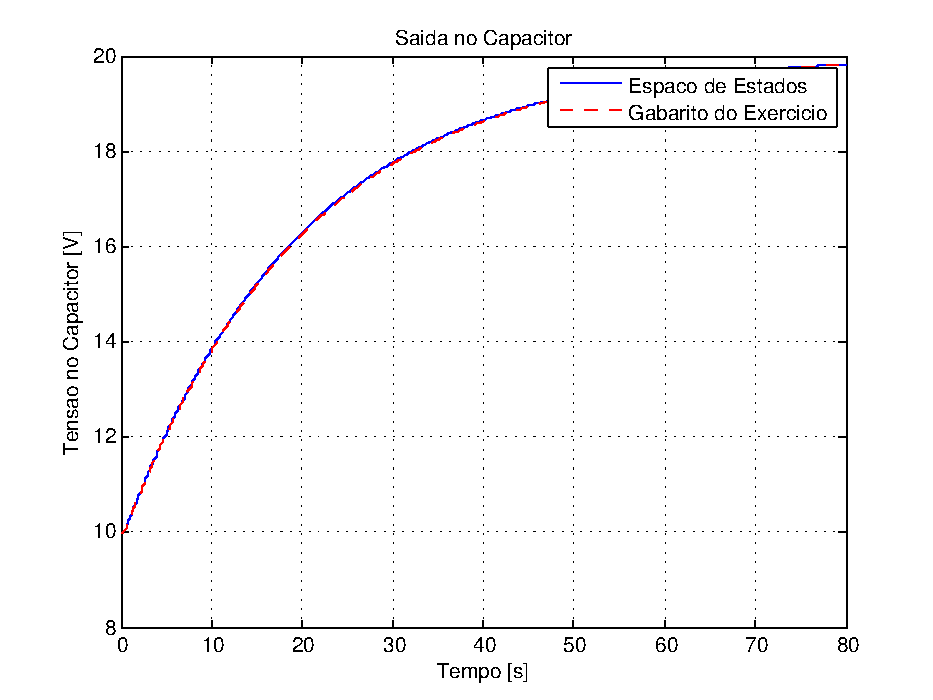
\includegraphics[width=0.85\textwidth]{images/plots/plot_8_33_y1.pdf}
    \caption{\label{plot:8.33_y1} Saída $ y_1 $ do Exercício 8.33}
\end{figure}

Nessa saída, observa-se que há uma ótima sobreposição de saída do Espaço de Estados e da função fornecida pelo gabarito da questão.
\clearpage
\begin{figure}[h!]
    \centering
    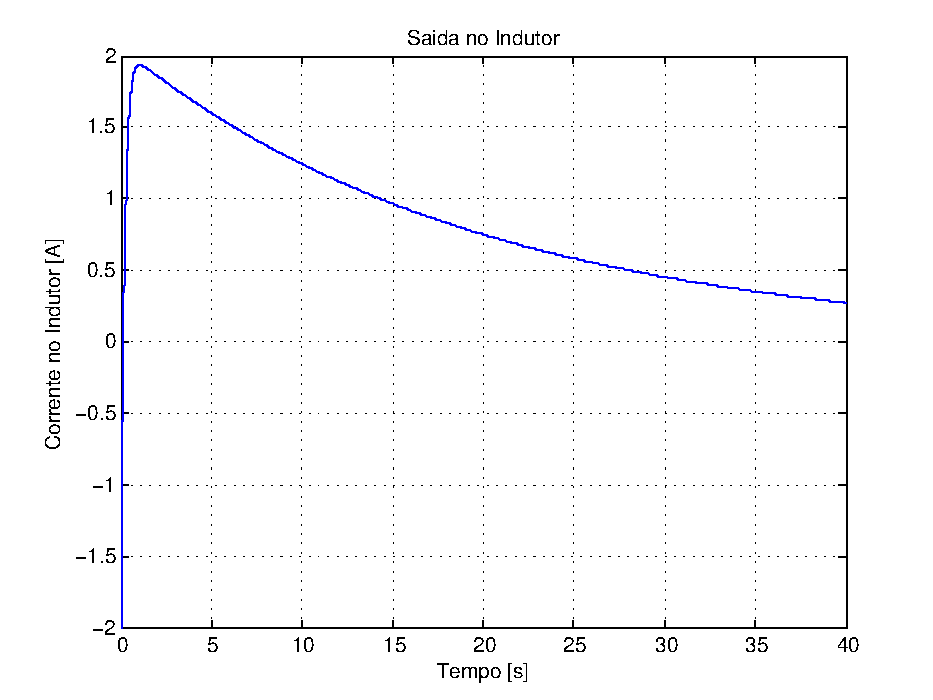
\includegraphics[width=0.85\textwidth]{images/plots/plot_8_33_y2.pdf}
    \caption{\label{plot:8.33_y2} Saída $ y_2 $ do Exercício 8.33}
\end{figure}

Na figura acima, observa-se que a corrente no indutor parte de $ -2\text{A} $ e chega até o regime permanente esperado de $ 0\text{A} $.

\begin{figure}[h!]
    \centering
    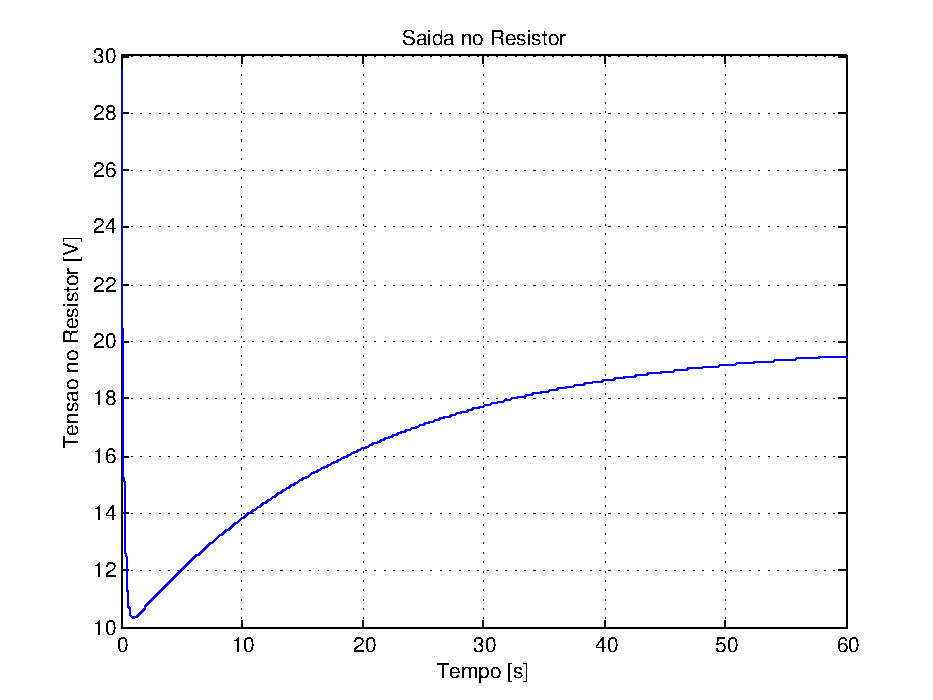
\includegraphics[width=0.85\textwidth]{images/plots/plot_8_33_y3.pdf}
    \caption{\label{plot:8.33_y3} Saída $ y_3 $ do Exercício 8.33}
\end{figure}

Por fim, é observável que a figura acima representa bem o comportamento da tensão sobre o resistor. Partindo de $ 30\text{V} $ e chegando no regime
permanente de $ 20 \text{V} $.

\begin{center}
    \[ \scalebox{3}{$ * $} \]
\end{center}

\subsection{Simulação do Exercício 8.38.1}
Começando novamente pela representação gráfica da resposta do próprio exercício:
$$ I_L(t) = \left\{8 + e^{-400t}\left[2\cos(300t) + 11\sin(300t)\right]\right\}\text{A}, t > 0 $$

Agora, partindo da expressão \ref{eq:8.38.1_sol}, o código para comparar as respostas e expressar as outras saídas é o seguinte:
\lstinputlisting[caption=Exercício 8.38.1,
                captionpos=b,
                basicstyle=\footnotesize,
                numbers=left,
                columns=flexible,
                xleftmargin=26pt,
                frame=single,
                framexleftmargin=22pt,
                aboveskip=15pt,
                breaklines=true,
                language=Matlab]
                {code/ex_8_38_1.m}

A partir daí, foram construídos os seguintes gráficos:
\begin{figure}[h!]
    \centering
    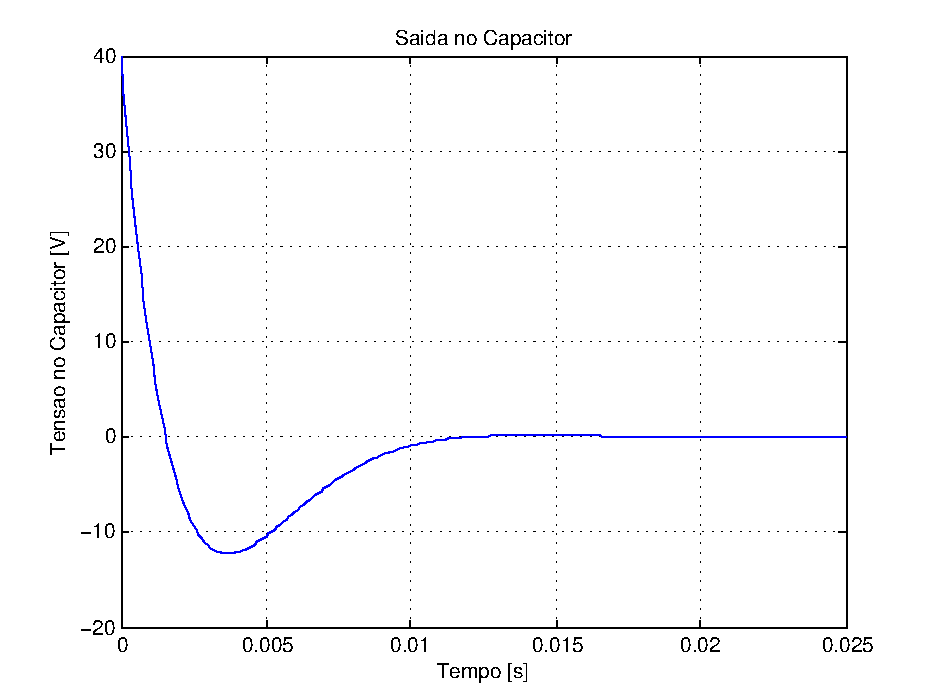
\includegraphics[width=0.85\textwidth]{images/plots/plot_8_38_1_y1.pdf}
    \caption{\label{plot:8.38.1_y1} Saída $ y_1 $ do Exercício 8.38.1}
\end{figure}

Aqui, na tensão do capacitor, é observável que ela começa nos $ 40\text{V} $, tem comportamento senoidal amortecido e
acaba na mesma tensão do indutor carregado, $ 0\text{V} $.
\clearpage
\begin{figure}[h!]
    \centering
    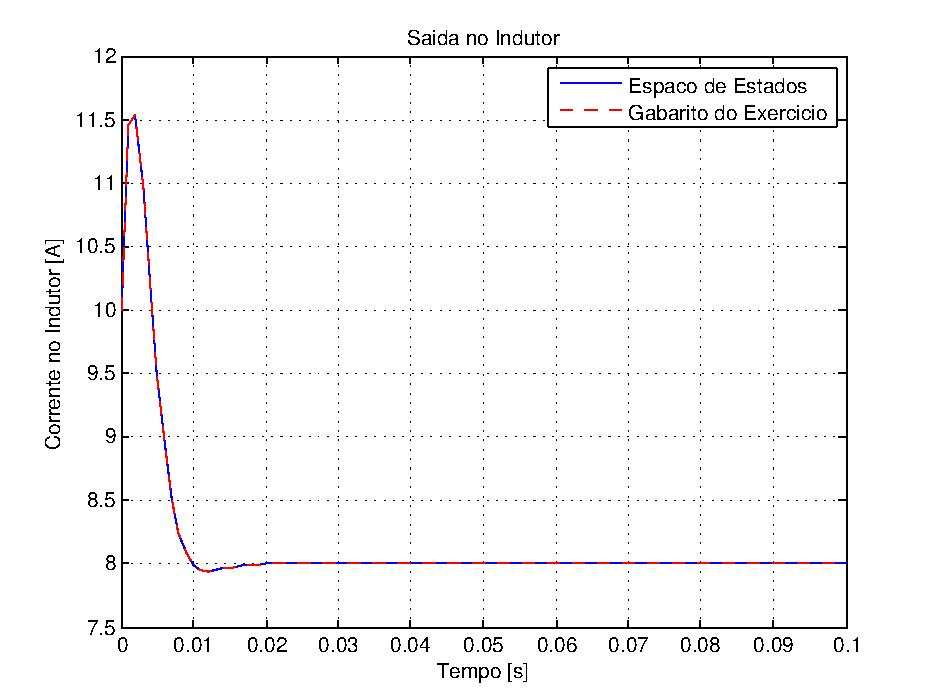
\includegraphics[width=0.85\textwidth]{images/plots/plot_8_38_1_y2.pdf}
    \caption{\label{plot:8.38.1_y2} Saída $ y_2 $ do Exercício 8.38.1}
\end{figure}

Nessa figura, é visível que há uma ótima sobreposição entre os resultados da função do gabarito com a resposta em Representação de Espaço de Estados, confirmando
que a corrente começa em $ 10\text{A} $ e acaba em $ 8\text{A} $, com comportamento senoidal amortecido.

\begin{figure}[h!]
    \centering
    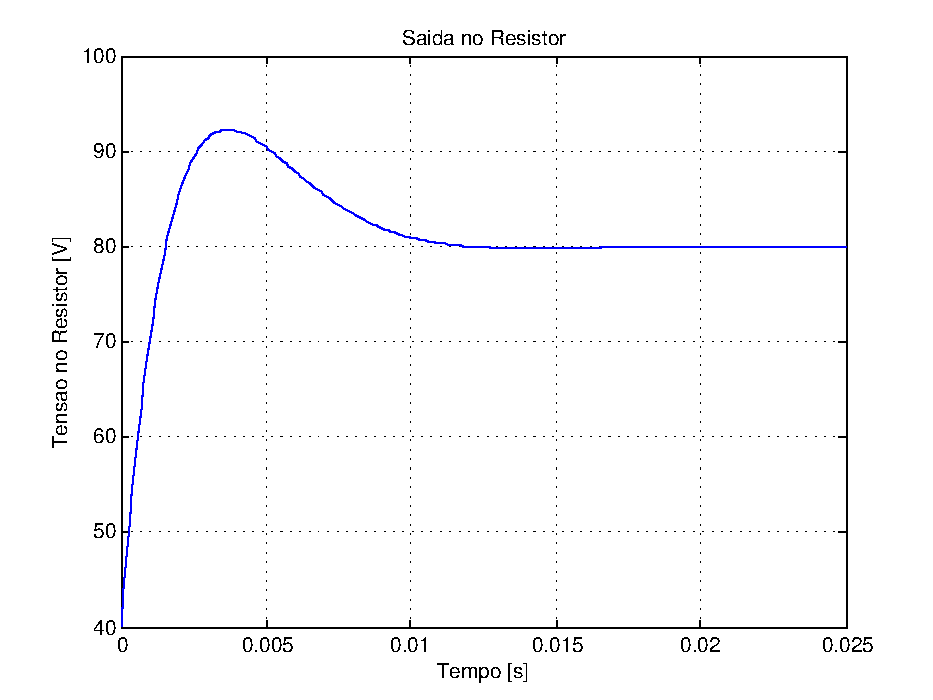
\includegraphics[width=0.85\textwidth]{images/plots/plot_8_38_1_y3.pdf}
    \caption{\label{plot:8.38.1_y3} Saída $ y_3 $ do Exercício 8.38.1}
\end{figure}

Por fim, é observável que a figura acima representa bem o comportamento da tensão sobre o resistor. Partindo de $ 40\text{V} $ e chegando no regime
permanente de $ 80 \text{V} $. No intervalo central, se comportando com o mesmo tipo de oscilação que as outras grandezas acima.

\subsection{Simulação do Exercício 8.38.2}
A resposta dada pelo exercício é:
$$ I_L(t) = \left(e^{-4,431t} + e^{-0,903t}\right)\text{A}, t > 0 $$

O programa utilizado para gerar os resultados gráficos, contando com \ref{eq:8.38.2_sol}, está a seguir:

\subsection{Simulação do Exercício 8.39}
Por fim, o exercício fornece o seguinte comportamento esperado para uma de suas grandezas:
$$ V_C(t) = \left(-6 -0,\!02e^{-47,83t} + 6,\!02e^{-0,17t}\right)\text{V}, t > 0 $$

A seguir, baseado em \ref{eq:8.39_sol}, segue o código para gerar os gráficos das respostas:

\section{Conclusões Finais}

\end{document}